\documentclass{article}
\usepackage{graphicx}
\usepackage{wrapfig}
\graphicspath{{./images/}}

\begin{document}
\author{Hawley, Adam}
\title{Lecture 3: Photometric Image Formation\\Part 1}
\maketitle
\section{Types of Sensor}
There are many different types of sensors used in computer vision:
\begin{itemize}
	\item Optical
	\begin{itemize} \item CCD, Photodiodes, Photomultipliers \end{itemize}
	\item Infra-red (thermal imaging cameras)
	\begin{itemize} \item CCD (Cooled), Photodiodes \end{itemize}
	\item Synthetic Aperture Radaaar (SAR)
	\begin{itemize} \item Radar, Antenna \end{itemize}
	\item Range Sensors
	\begin{itemize} \item Laser \& Photodiode \end{itemize}
	\item MRI
	\begin{itemize} \item Magnetic field gradients applied causing production of rotating magnetic field which can be measured. \end{itemize}
	\item PET/CAT
	\begin{itemize} \item Simulated radiation emission via magnetic field or radio isotope. \end{itemize}
\end{itemize}
\section{From Light to Images}
\subsection{Definitions}
\begin{itemize}
	\item {\textit{\textbf {Irradiance}}}: power incident on a surface (power per unit area).
	\item {\textit{\textbf {Radiance}}}: power travelling from a source (power per unit solid angle per unit projected source area).
\end{itemize}
\subsection{Charge-Coupled Devices}
The most common devixe for digitising image information is a charge-coupled device (CCD). 
They are made up of a square array of solid-state capacitors: \\
\begin{figure}[h]
	\centering
	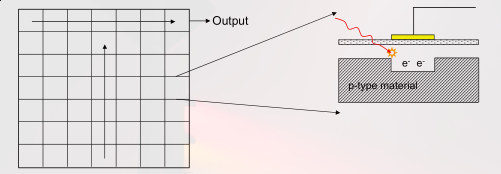
\includegraphics[width=\textwidth]{ccd.png}
	\caption{The flow of electrons inside a CCD}
	\label{fig:CCD}
\end{figure} \\
From the photo-electric effect photons of light knock out electrons from the upper plate and hence charge accumulates in the electron capture ``{\it wells}".
Using a shift register, capacitors tranfer their contents to the appropriate neighbour.
The final capacitor dumps the charge for each capacitor into the analogue-digital converter (ADC).
The dump happens once for each capacitor until the contents of each one has been read. \\
\begin{wrapfigure}{l}{0.25\textwidth}
	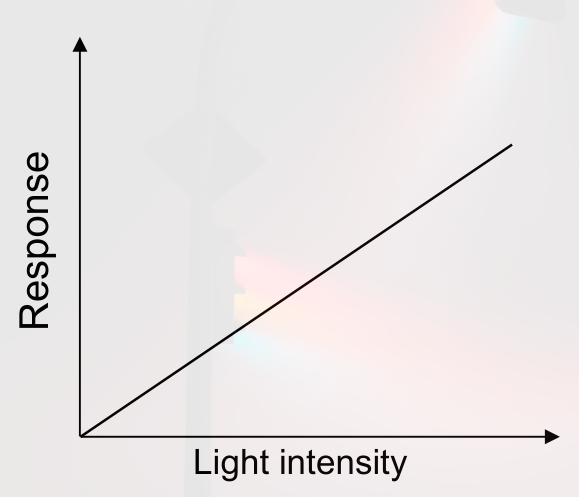
\includegraphics[width=0.25\textwidth]{ccdResponse1.png}
	\caption{Ideal response of a CCD}
	\label{fig:ccdResponse1}
\end{wrapfigure}
The ideal reading from a CCD would be as simple as ``$output = gain\cdot input$". See figure \ref{fig:ccdResponse1}. \\
\begin{wrapfigure}{l}{0.25\textwidth}
	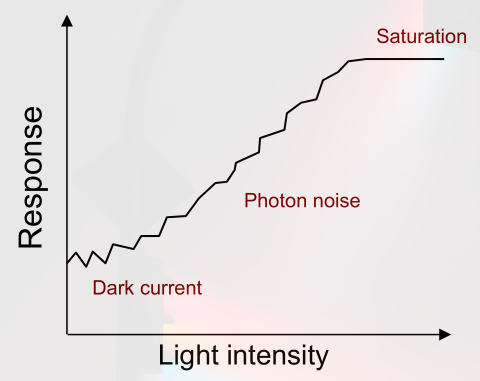
\includegraphics[width=0.25\textwidth]{ccdResponse2.png}
	\caption{Typical response of a CCD}
	\label{fig:ccdResponse2}
\end{wrapfigure}
However, a typical reading from a CCD also includes bias and noise.
(``$output = gain \cdot input + bias + noise$'')
The noise mostly comes from the following sources:
\begin{itemize}
	\item Dark Cuttent - Thermal noise.
	\item Photon Noise - Quantum noise.
	\item Quantisation of pixels.
	\item Amplifier
\end{itemize}
See figure \ref{fig:ccdResponse2}.
\end{document}
